\clearpage
%//==============================--@--==============================//%
\vspace{-1em}
\subsection{P6 | Desenvolvimento de resistência nas células cancerígenas}
\label{subsec:P6}

O processo de modelação do desenvolvimento de resistência nas células cancerígenas é de natureza não trivial. A resistência adquirida afeta, mediante vários vetores de ataque, o \hyperref[subsec:P2]{modelo farmacodinâmico} (\textit{drug-concentration response}), e é inerentemente dependente do corpo hospedeiro:

\begin{quote}
    \textit{``Resistance to therapy results from host factors, such as poor
    absorption or rapid metabolism, or epigenetic alterations in the cancer cells.''}\cite{teles_2017}
\end{quote}

Consequentemente, desenvolveram-se dois modelos baseados na interação \textit{drug-receptor}, de nomes \textbf{"Antagónico Competitivo"} e \textbf{"Antagónico Não Competitivo"}, cuja descrição é sucintamente inframencionada:

\begin{figure}[ht] 
    \begin{subfigure}[b]{0.5\linewidth}
        \hfill
        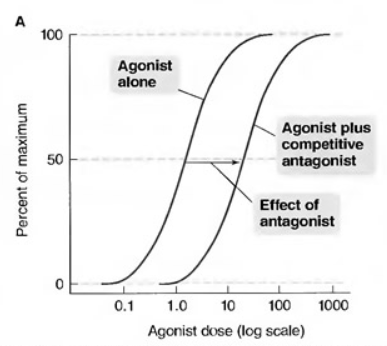
\includegraphics[width=0.8\linewidth]{img/perguntas/P6/P6-Competitive.png}
        \vspace{1ex}
        \hspace*{7.5em}\begin{minipage}{0.5\linewidth}
            \caption{Modelo competitivo} 
            \label{fig:LABEL-competitive} 
        \end{minipage}
    \end{subfigure}%% 
    \quad
    \begin{subfigure}[b]{0.5\linewidth}
        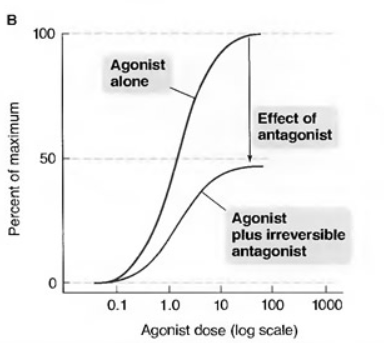
\includegraphics[width=0.8\linewidth]{img/perguntas/P6/P6-NCompetitive.png} 
        \vspace{1ex}
        \hspace*{3.5em}\begin{minipage}{0.5\linewidth}
            \caption{Modelo não competitivo} 
            \label{fig:LABEL-ncompetitive} 
        \end{minipage}
    \end{subfigure}
    \caption{\textit{Drug concentration-response} com efeito antagónico\cite{10.1093/bjaceaccp/mkh049}.}
\end{figure}

 \hyperref[fig:LABEL-competitive]{\textbf{A | Modelo Competitivo}}: A resistência compete com a ação do fármaco no recetor. O aumento de administração de fármaco detém o efeito da resistência (\textit{``(...) can be overcome by increasing the dose of the agonist [fármaco].''}\cite{10.1093/bjaceaccp/mkh049})
 
 \hspace*{1.25 em}\raisebox{0.2 em}{$\drsh$} \textbf{Efeito} $\rightarrow$ A curva \textit{drug-concentration response} sofre um desvio para a direita, mediante o incremento do parâmetro $C_{50}$.\footnotemark[9]

\begin{equation}
    \textbf{\hyperref[eq:modelo-PD]{Modelo de efeito (2)} adaptado} \rightarrow u \delequal \frac{C_p(t)}{(1 + r(t))\cdot C_{50} + C_p(t)}
\end{equation}

\hyperref[fig:LABEL-ncompetitive]{\textbf{B | Modelo não Competitivo}}: A resistência inibe a ação do fármaco no recetor. 
 
 \hspace*{1.25 em}\raisebox{0.2 em}{$\drsh$} \textbf{Efeito} $\rightarrow$ O efeito do fármaco é progressivamente menor, a curva de \textit{drug-concentration response} sofre um \textit{shrink}, \textit{``The actions of a non-competitive antagonist cannot be overcome by increasing the dose (...)''}.\cite{10.1093/bjaceaccp/mkh049}
 
\begin{equation}
    \textbf{\hyperref[eq:modelo-PD]{Modelo de efeito (2)} adaptado} \rightarrow u \delequal \frac{1}{1 + r(t)}\cdot\frac{C_p(t)}{C_{50} + C_p(t)}
\end{equation}

O modelo da resistência, $r(t)$, procura respresentar o efeito que baixas concentrações de fármaco induzem nas mutações das células cancerígenas. O modelo desenvolvido, bem como a sua representação gráfica encontram-se abaixo:
%//==============================--@--==============================//%
\footnotetext[9]{\textit{``Acquired resistance can be incorporated in the model by increasing the $C_{50}$ parameter from PD (...), since it will directly decrease the drug effect.''}\cite{teles_2017}}
%//==============================--@--==============================//%
\newpage
\begin{wrapfigure}{l}{0.5\textwidth}
    \centering
    \vspace{0.55 em}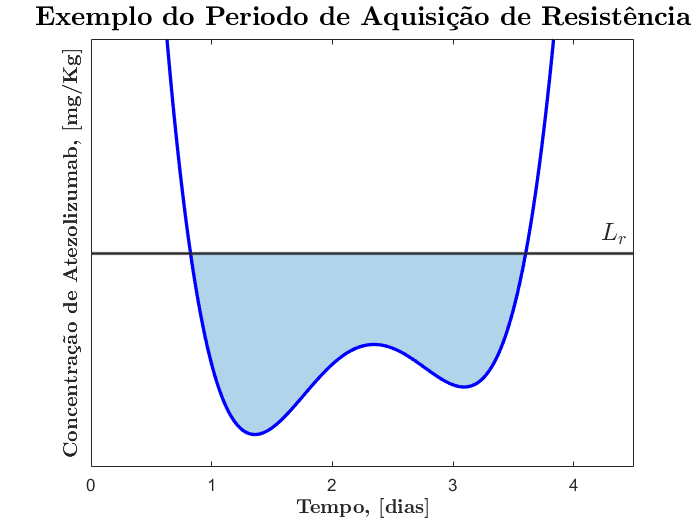
\includegraphics[width=0.5\textwidth]{img/perguntas/P6/P6-AreaMutation.png}
    \caption{Representação gráfica da área de desenvolvimento de resistência, a \textcolor{cyan}{azul}. A curva a \textcolor{blue}{azul escuro} representa uma curva de concentração.}
    \label{fig:P6-area}
\end{wrapfigure}

$$
    \xrightarrow[]{}
    \begin{cases}
        r(t) = K_r \cdot \int_{0}^{t} \max[0, L_r - C_p(\tau)] \,d\tau \\
        \dot{r}(t) = K_r \cdot \max[0, L_r - C_p(t)]
    \end{cases}
$$

Onde $K_r$ é o coeficiente de capacidade de mutação do tumor\cite{toxicity-lemos} e a resistência é apenas desenvolvida abaixo de uma linha de \textit{Threshold}, $L_r$ onde \textit{``(...) the driving tolerance is directly proportional to the intensities of past exposures (...)''}\cite{Porchet1988-bs} $\rightarrow$ cálculo da área de concentração abaixo do limite de \textit{Threshold}.

A simulação dos modelos foi realizada mediante um exemplo de terapia real de nome \textit{Intravenous (IV) Bolus Therapy}\footnotemark[10]\cite{teles_2017}:

\vphantom{Experiência 123}

\vphantom{Experiência 123}

\vspace{-2em}
\begin{figure}[ht]
    \begin{subfigure}[b]{0.5\linewidth}
        \centering
        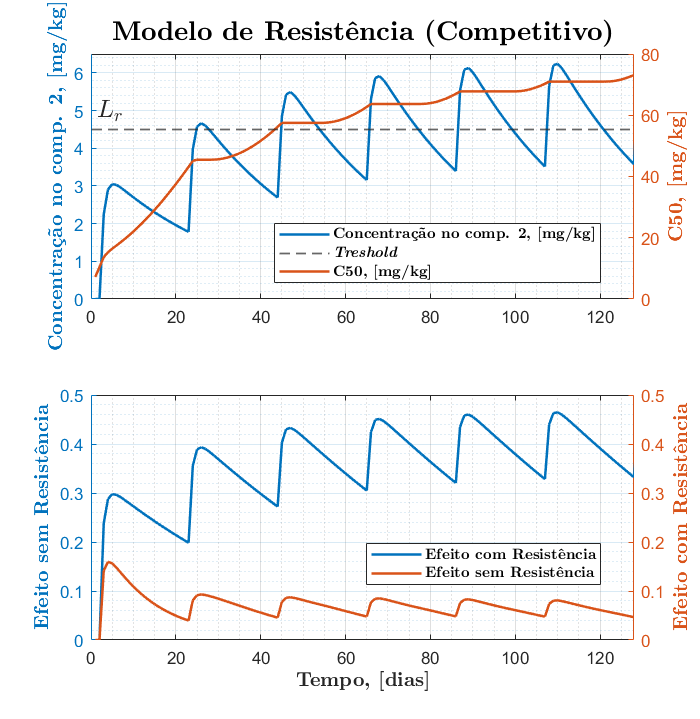
\includegraphics[width=0.9\linewidth]{img/perguntas/P6/P6-compete.png}
        \caption{Modelo de resistência antagonista competitiva.} 
        \label{fig:LABEL-compete} 
        %\vspace{1ex}
    \end{subfigure}%% 
    \begin{subfigure}[b]{0.5\linewidth}
        \centering
        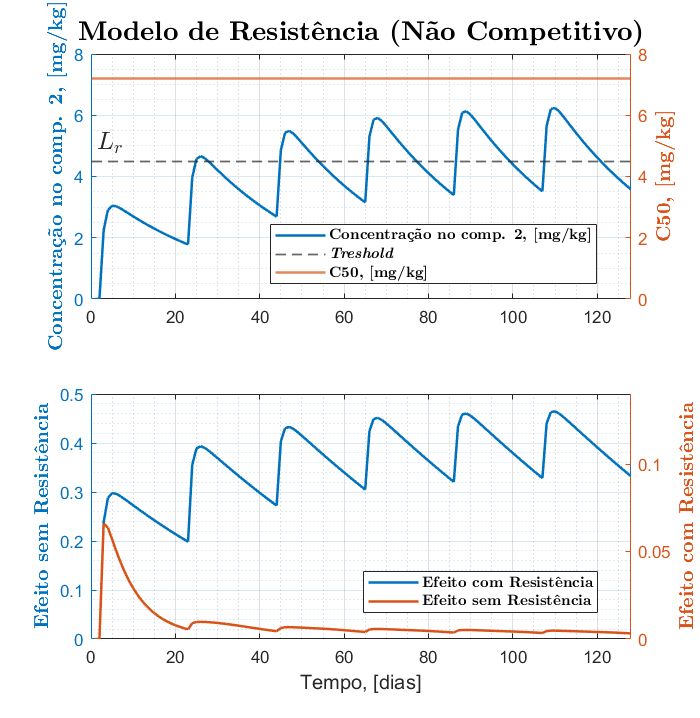
\includegraphics[width=0.9\linewidth]{img/perguntas/P6/P6-ncompete.png} 
        \caption{Modelo de resistência antagonista não competitiva.} 
        \label{fig:LABEL-ncompete} 
        %\vspace{1ex}
    \end{subfigure} 
    \caption{Concentração no compartimento de efeito ($C_p$), evolução do parâmetro $C_{50}$ e comparação dos efeitos sem resistência e com resistência para ambos os modelos para a terapia de parâmetros.}
\end{figure}

\vskip -0.5em

\textbf{(a)} $\rightarrow$ Para o modelo competitivo \textbf{o parâmetro $C_{50}$ incrementa apenas quando a concentração no compartimento de efeito é inferior à linha de \textit{Threshold}} (a integração em $r(t)$ é apenas realizada quando esta condição se verifica), de notar o \textbf{caráter oscilatório da regressão} (correspondente a iterações de incremento e estabilidade). \textbf{O efeito possui} \textbf{uma redução significativa} relativamente ao efeito não limitado pela resistência adquirida (consequência dos sucessivos desvios da curva de Hill).

\vskip 0.5em
\textbf{(b)} $\rightarrow$ Para o modelo não competitivo realça-se a \textbf{mitigação acentuada do efeito do fármaco}, quando comparado ao modelo anterior, coerente com o já discutido acima: Este modelo inibe o efeito, esta inibição não é solúvel por meio de incremento de concentração (\textbf{a curva de \textit{drug-concentration response}, sofre constrangimentos sucessivos, aproximando-se da nulidade)}.


%//==============================--@--==============================//%
\footnotetext[10]{$T = 21$d, dose $= 20$ mg/kg, para $K_r = 0.1$ e \textit{Threshold}$ = 4.5$}
%//==============================--@--==============================//%

\begin{wrapfigure}{l}{0.55\textwidth}
    \centering
    \vspace{-0.5 em}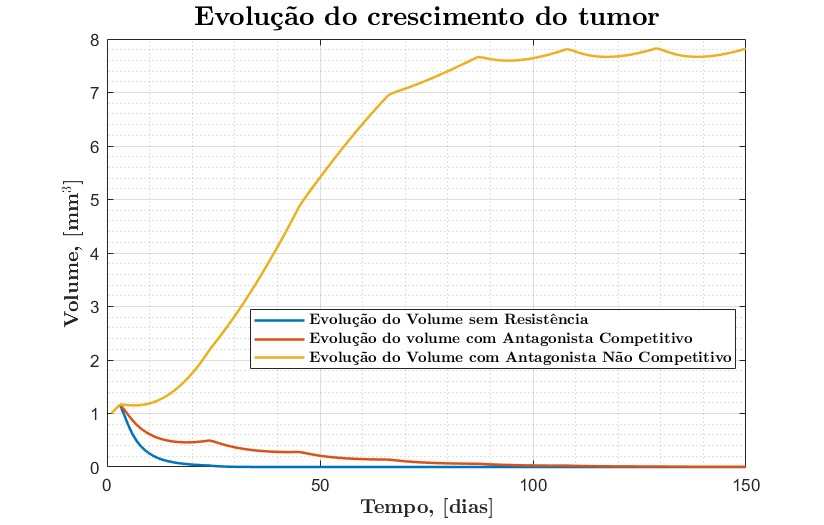
\includegraphics[width=0.55\textwidth]{img/perguntas/P6/P6-TumorGrowth.png}
    \caption{Comparação das 3 evoluções do tumor mediante o modelo de resistência projetado.}
    \label{fig:P6-volume}
\end{wrapfigure}

\vphantom{experiencia 123}
Supondo agora um \textit{Threshold} de 3.5, para o qual a concentração no compartimento de efeito é continuamente superior\footnotemark[11] (após algumas iterações de administração), duas conclusões são aparentes:

$\rightarrow$ A evolução do volume afetado pelo modelo antagonista competitivo é análoga à  evolução não afetada, possuindo apenas uma janela temporal mais alargada. Tal seria esperado: a resistência afeta a posição da curva de resposta do fármaco, mas não o seu \hyperref[eq:modelo-PD]{$u_{max}$}, $\pmb{\star}$ \textbf{a diminuição de volume é mais tardia}.

\vskip 0.5em

$\rightarrow$ A evolução do volume afetado pelo modelo antagonista não competitivo atinge um ponto de equilibrio, já discutido \hyperref[subsubsec:P3b]{secção P3}. Tal seria esperado: a resistência afeta o \hyperref[eq:modelo-PD]{$u_{max}$} da curva de resposta do fármaco, o seu efeito é sucessivamente e irreversivelmente menor.\\ $\pmb{\star}$ \textbf{Para mitigar este efeito seria necessário ser mais veloz que o desenvolvimento de resistência, o que equaciona em administrações iniciais de fármaco mais elevadas.}
%//==============================--@--==============================//%
\footnotetext[11]{O \textit{Threshold} previamente escolhido verificava-se sempre superior à concentração no compartimento de efeito de forma a demonstrar a evolução da atuação do fármaco. Em contexto real, supomos que a concentração de fármaco no corpo, após algumas administrações, consiga superar a criação de resistência. }